\section{Sectoral responses in every closure}\label{app:sectoral-panels}

The figures below (Figures~\ref{fig:sectoral-flex-f23} to \ref{fig:sectoral-fixed}) show what the nine distinct economies of the matrix make of the program described in Section~\ref{sec:io-bridge} at the level of the sector.
Each panel refers to one cell (the collapsed cells of Table~\ref{tab:results-matrix} share a panel). The left half compares, for each of the seven program sectors, the size of the impulse with the resulting change in gross output, in household consumption and in the sectoral price relative to the consumption basket. The right half places all 71 sectors in the output--price plane, with the program sectors marked by their numbers, or, where no price moves, ranks them by their output response.

Table~\ref{tab:program-sector-key} identifies the numbered program sectors in all panels.

\begin{table}[htbp]
\centering
\small
\begin{tabular}{rl}
\toprule
Number & Sector \\
\midrule
1 & Specialised construction works \\
2 & Rubber and plastics products \\
3 & Ceramic products, processed stone and clay \\
4 & Chemicals and chemical products \\
5 & Glass and glassware \\
6 & Machinery \\
7 & Electrical equipment \\
\bottomrule
\end{tabular}
\caption{Numbering of program sectors in
Figures~\ref{fig:sectoral-flex-f23}--\ref{fig:sectoral-fixed}. The numbers are
assigned in descending order of the sector's share in the program's bill, so
construction carries the number $1$ (63\% of the bill) and electrical equipment $7$
(1.3\%).}
\label{tab:program-sector-key}
\end{table}

\begin{figure}[htbp]
\centering
\begin{subfigure}{0.9\textwidth}
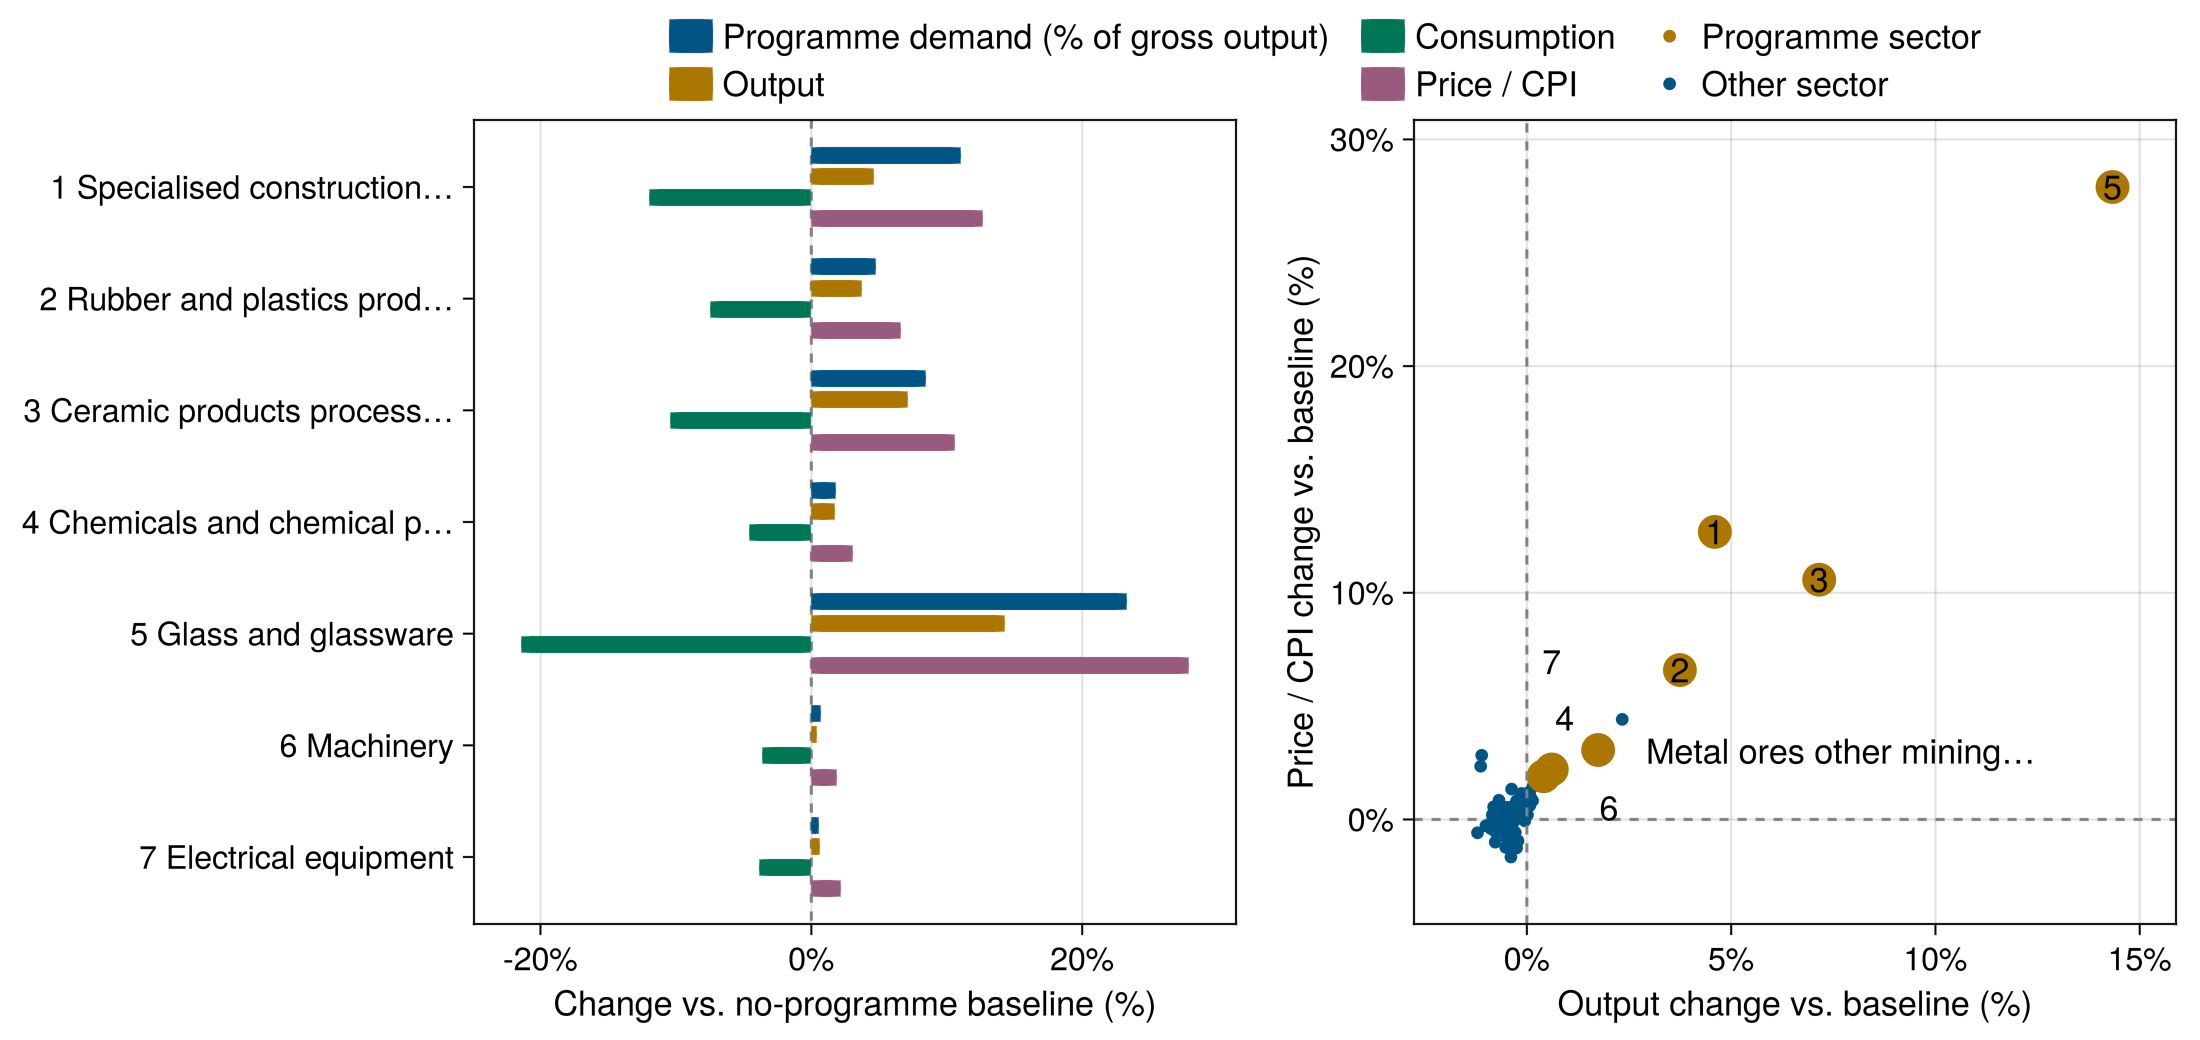
\includegraphics[width=\textwidth]{images/panel_5x3_BF_F2.png}
\caption{No-reallocation, F2/F3}
\end{subfigure}
\begin{subfigure}{0.9\textwidth}
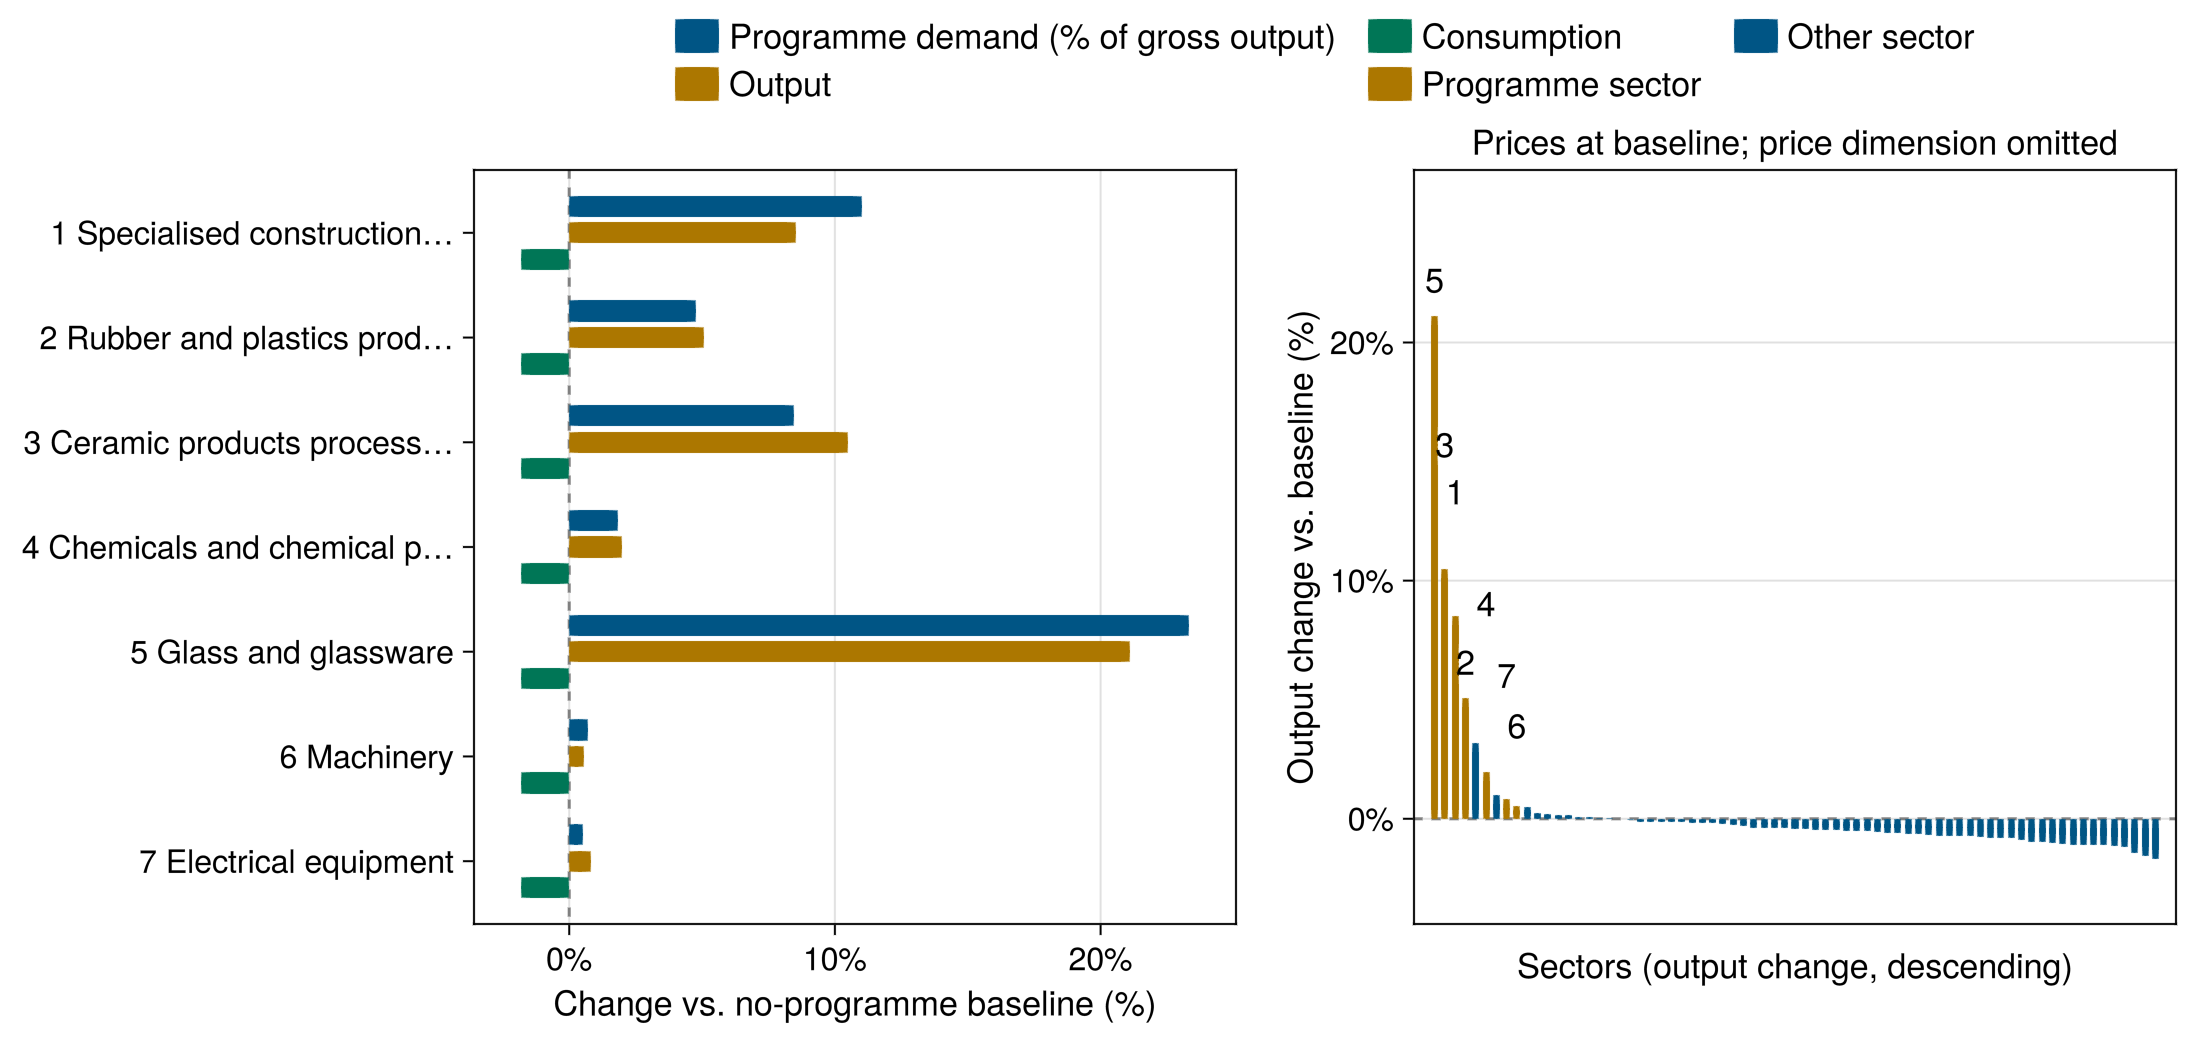
\includegraphics[width=\textwidth]{images/panel_5x3_ALPHA_F2.png}
\caption{Standard CGE, F2/F3}
\end{subfigure}
\begin{subfigure}{0.9\textwidth}
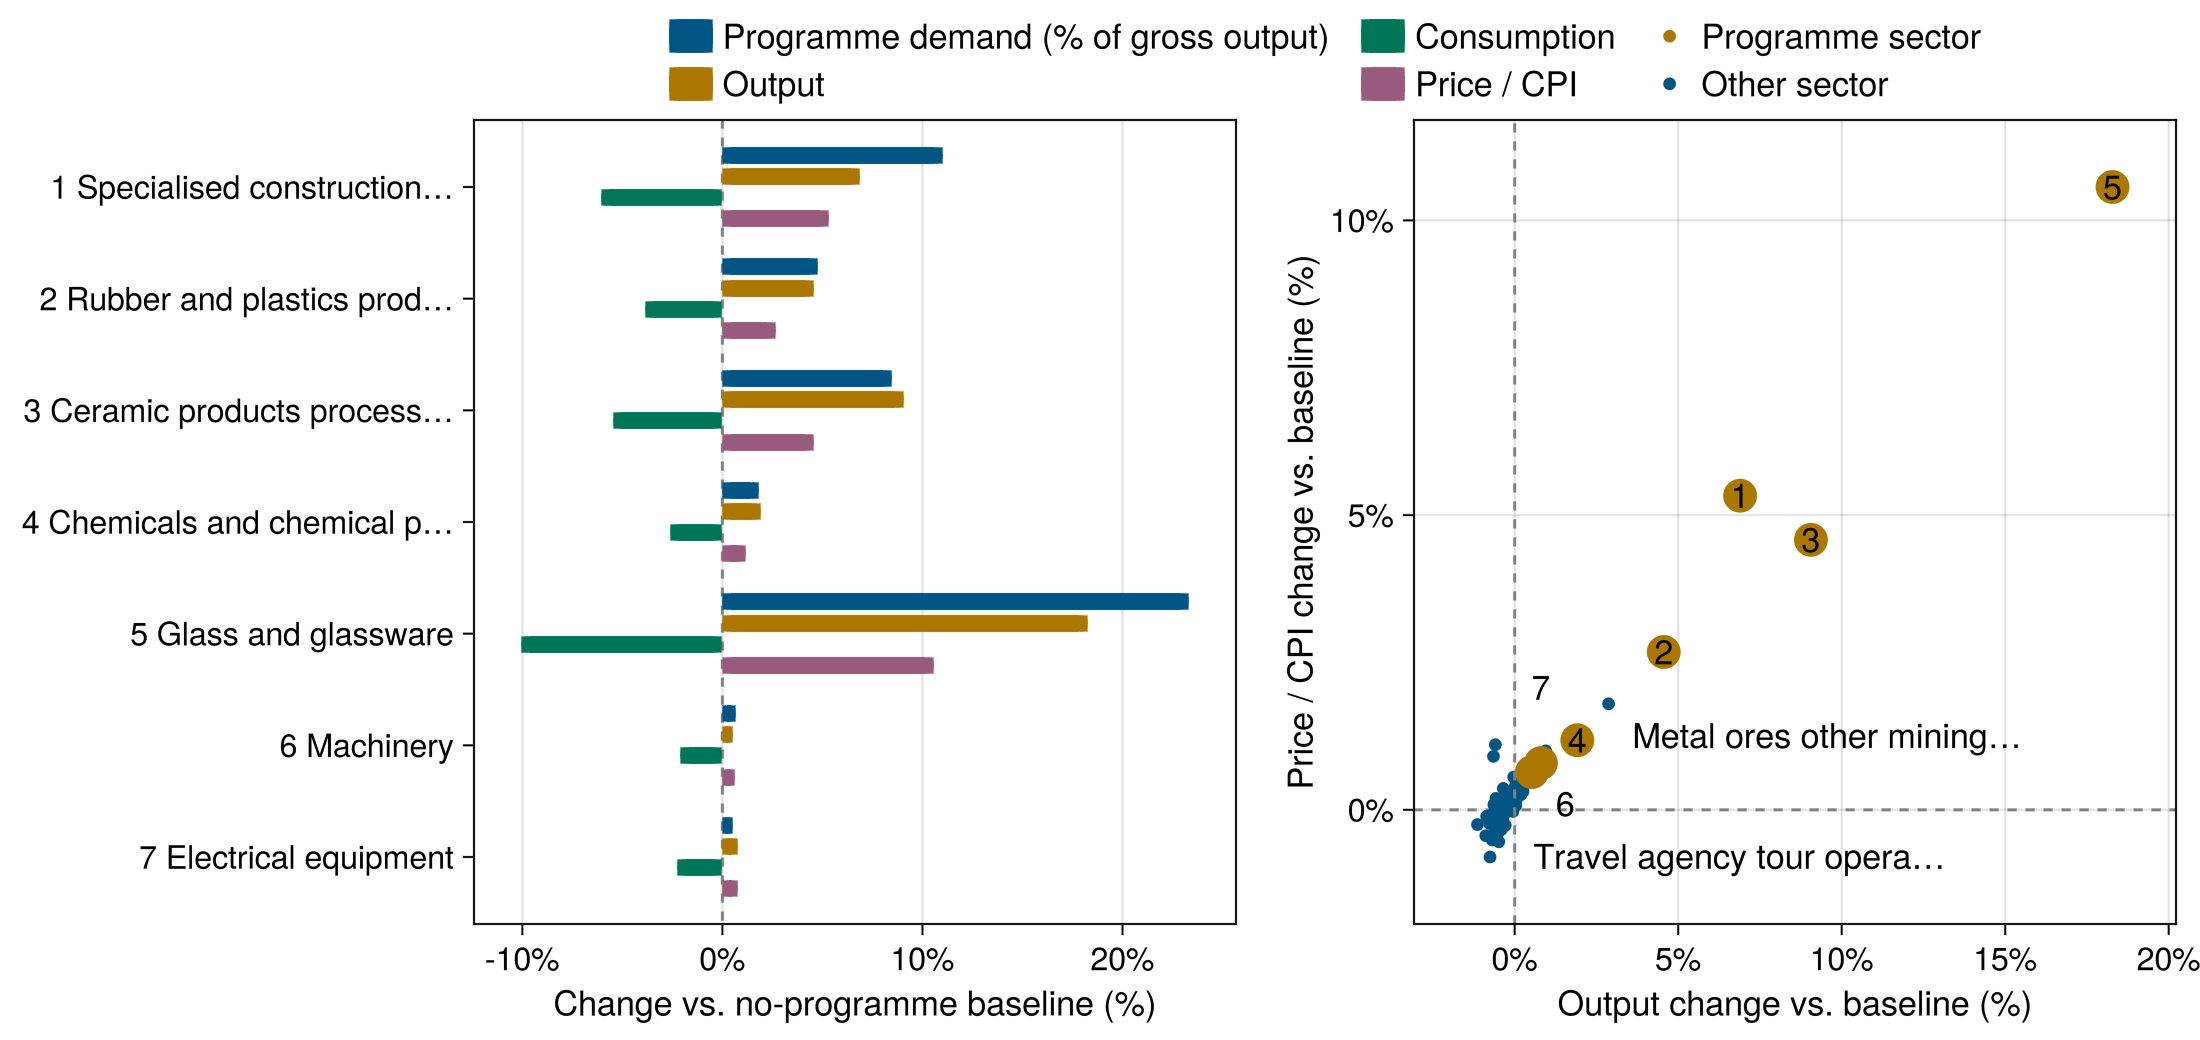
\includegraphics[width=\textwidth]{images/panel_5x3_BETA_F2.png}
\caption{Elastic labor supply ($\eta_s=0.5$), F2/F3}
\end{subfigure}
\caption{Sectoral responses under tax and external financing in the flexible-wage closures (F2 and F3 coincide). Layout as described above.}
\label{fig:sectoral-flex-f23}
\end{figure}

\begin{figure}[htbp]
\centering
\begin{subfigure}{0.9\textwidth}
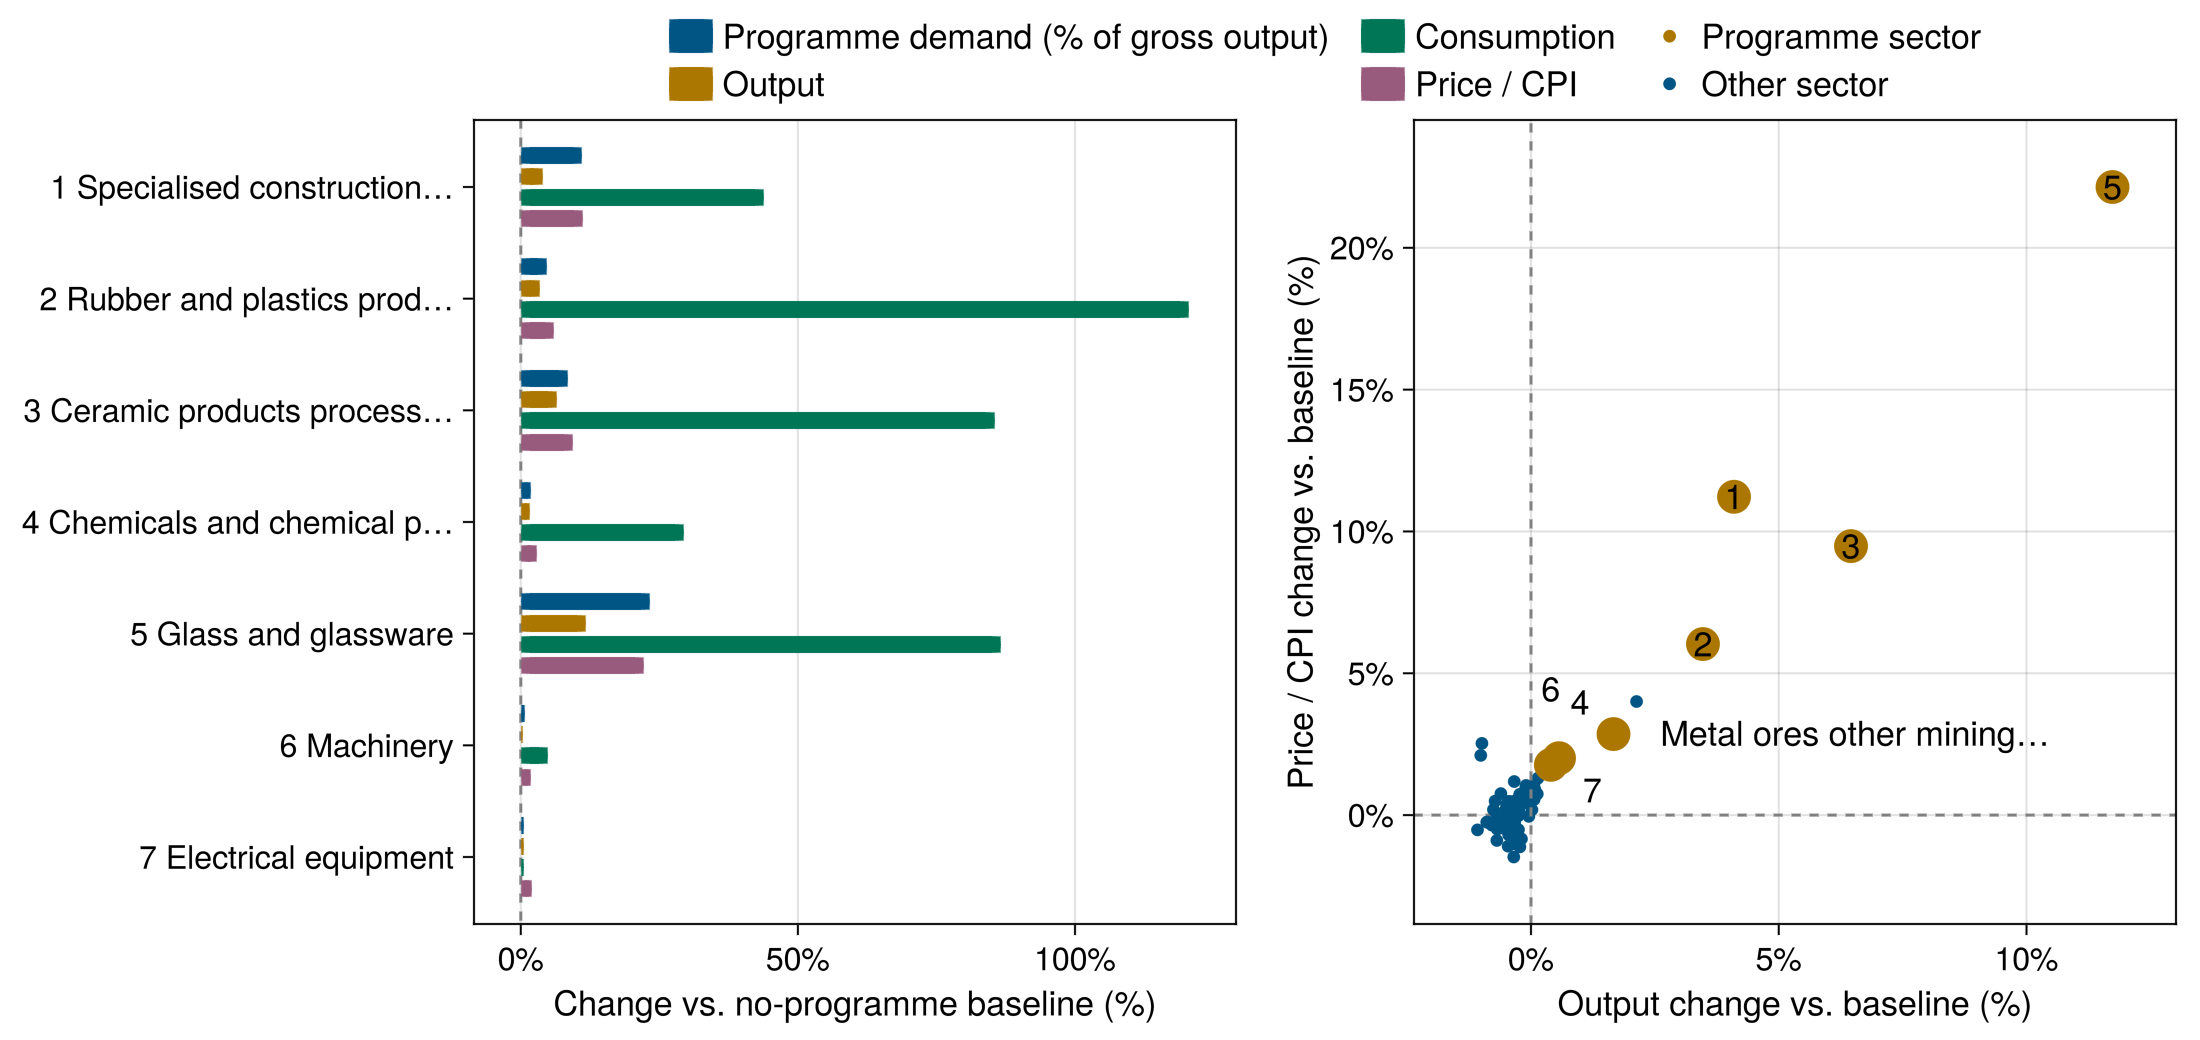
\includegraphics[width=\textwidth]{images/panel_5x3_BF_F1.png}
\caption{No-reallocation, F1}
\end{subfigure}
\begin{subfigure}{0.9\textwidth}
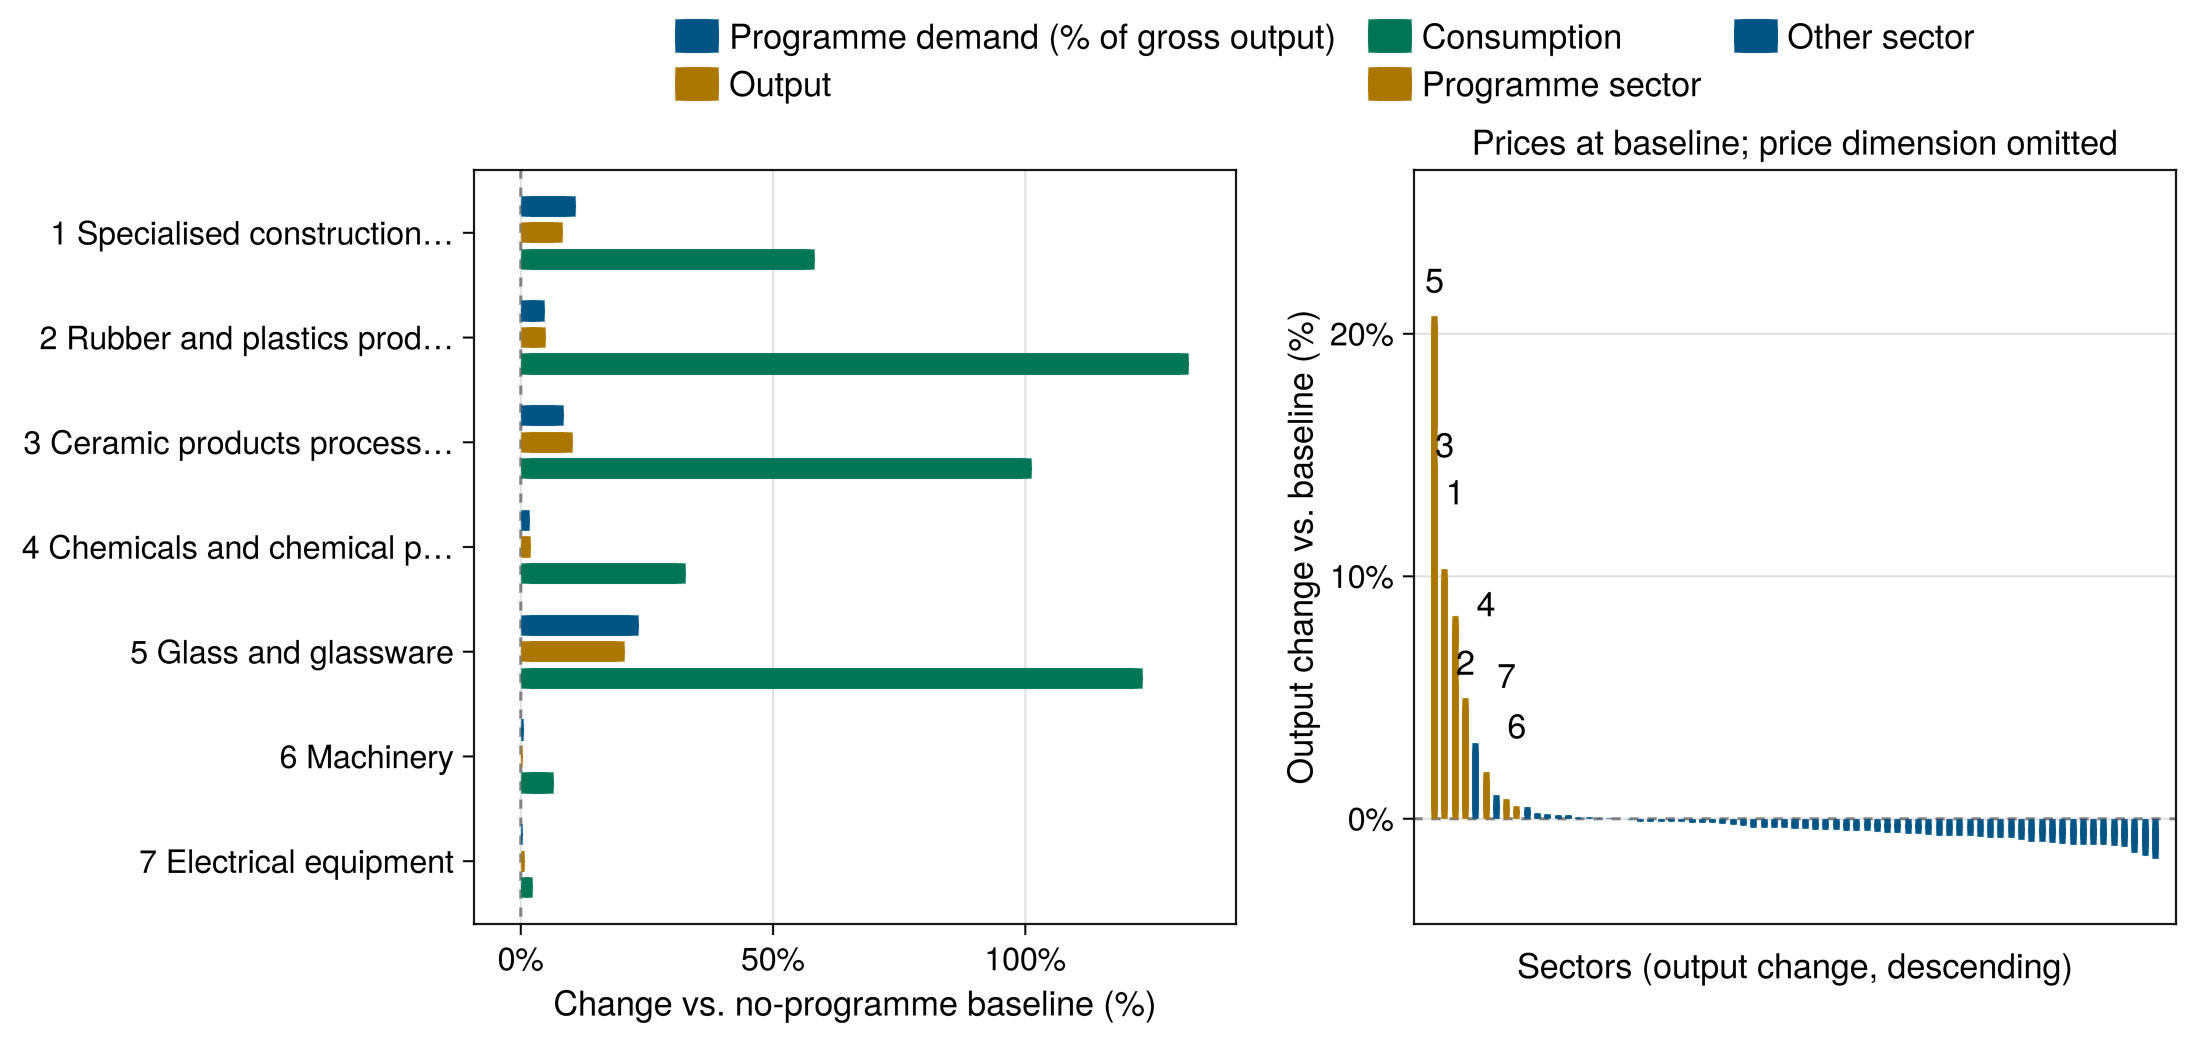
\includegraphics[width=\textwidth]{images/panel_5x3_ALPHA_F1.png}
\caption{Standard CGE, F1}
\end{subfigure}
\begin{subfigure}{0.9\textwidth}
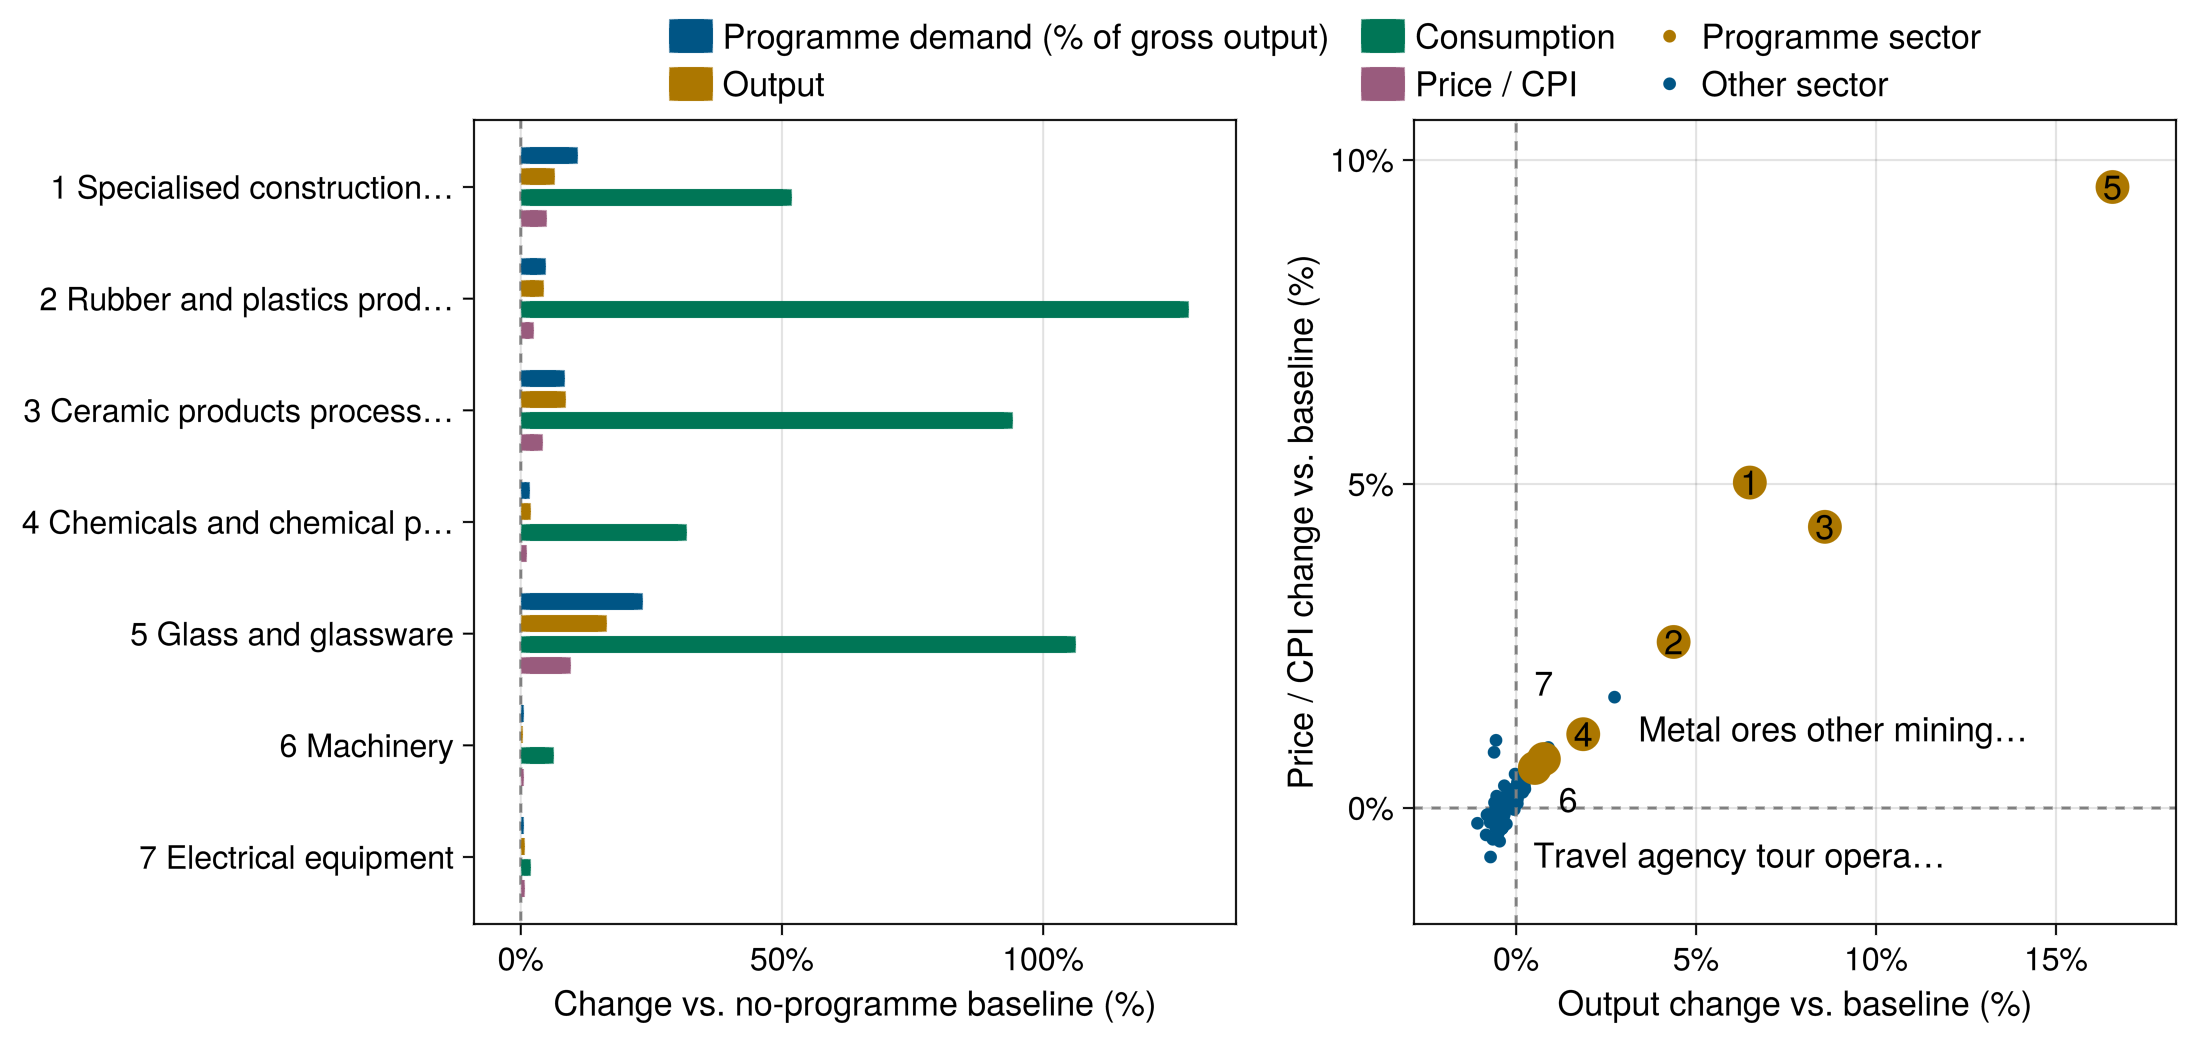
\includegraphics[width=\textwidth]{images/panel_5x3_BETA_F1.png}
\caption{Elastic labor supply ($\eta_s=0.5$), F1}
\end{subfigure}
\caption{Sectoral responses in the flexible-wage columns under the repurposing of consumption (F1). Layout as in Figure~\ref{fig:sectoral-flex-f23}.}
\label{fig:sectoral-flex-f1}
\end{figure}

\begin{figure}[htbp]
\centering
\begin{subfigure}{0.9\textwidth}
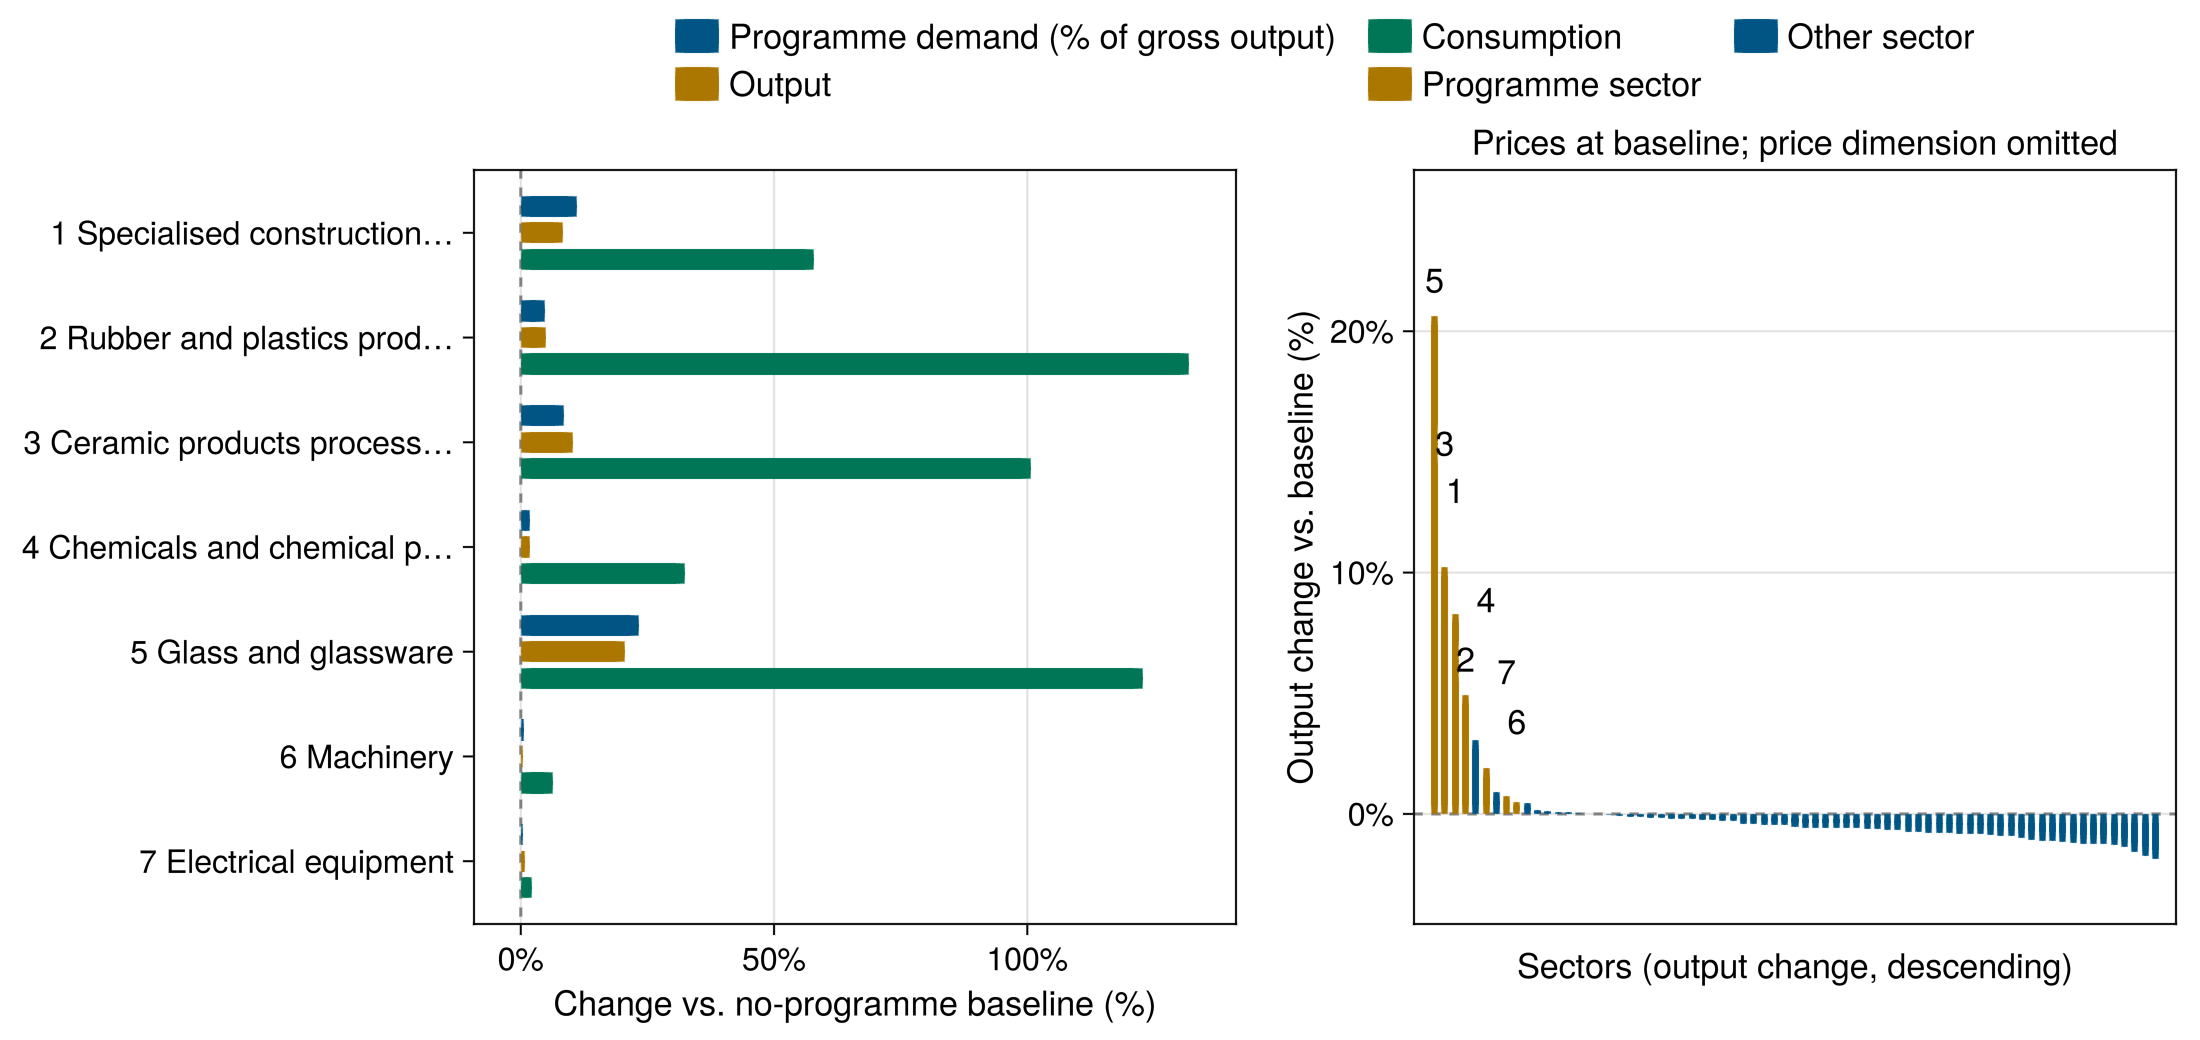
\includegraphics[width=\textwidth]{images/panel_5x3_GAMMA_F1.png}
\caption{Employment adjustment / Leontief, F1}
\end{subfigure}
\begin{subfigure}{0.9\textwidth}
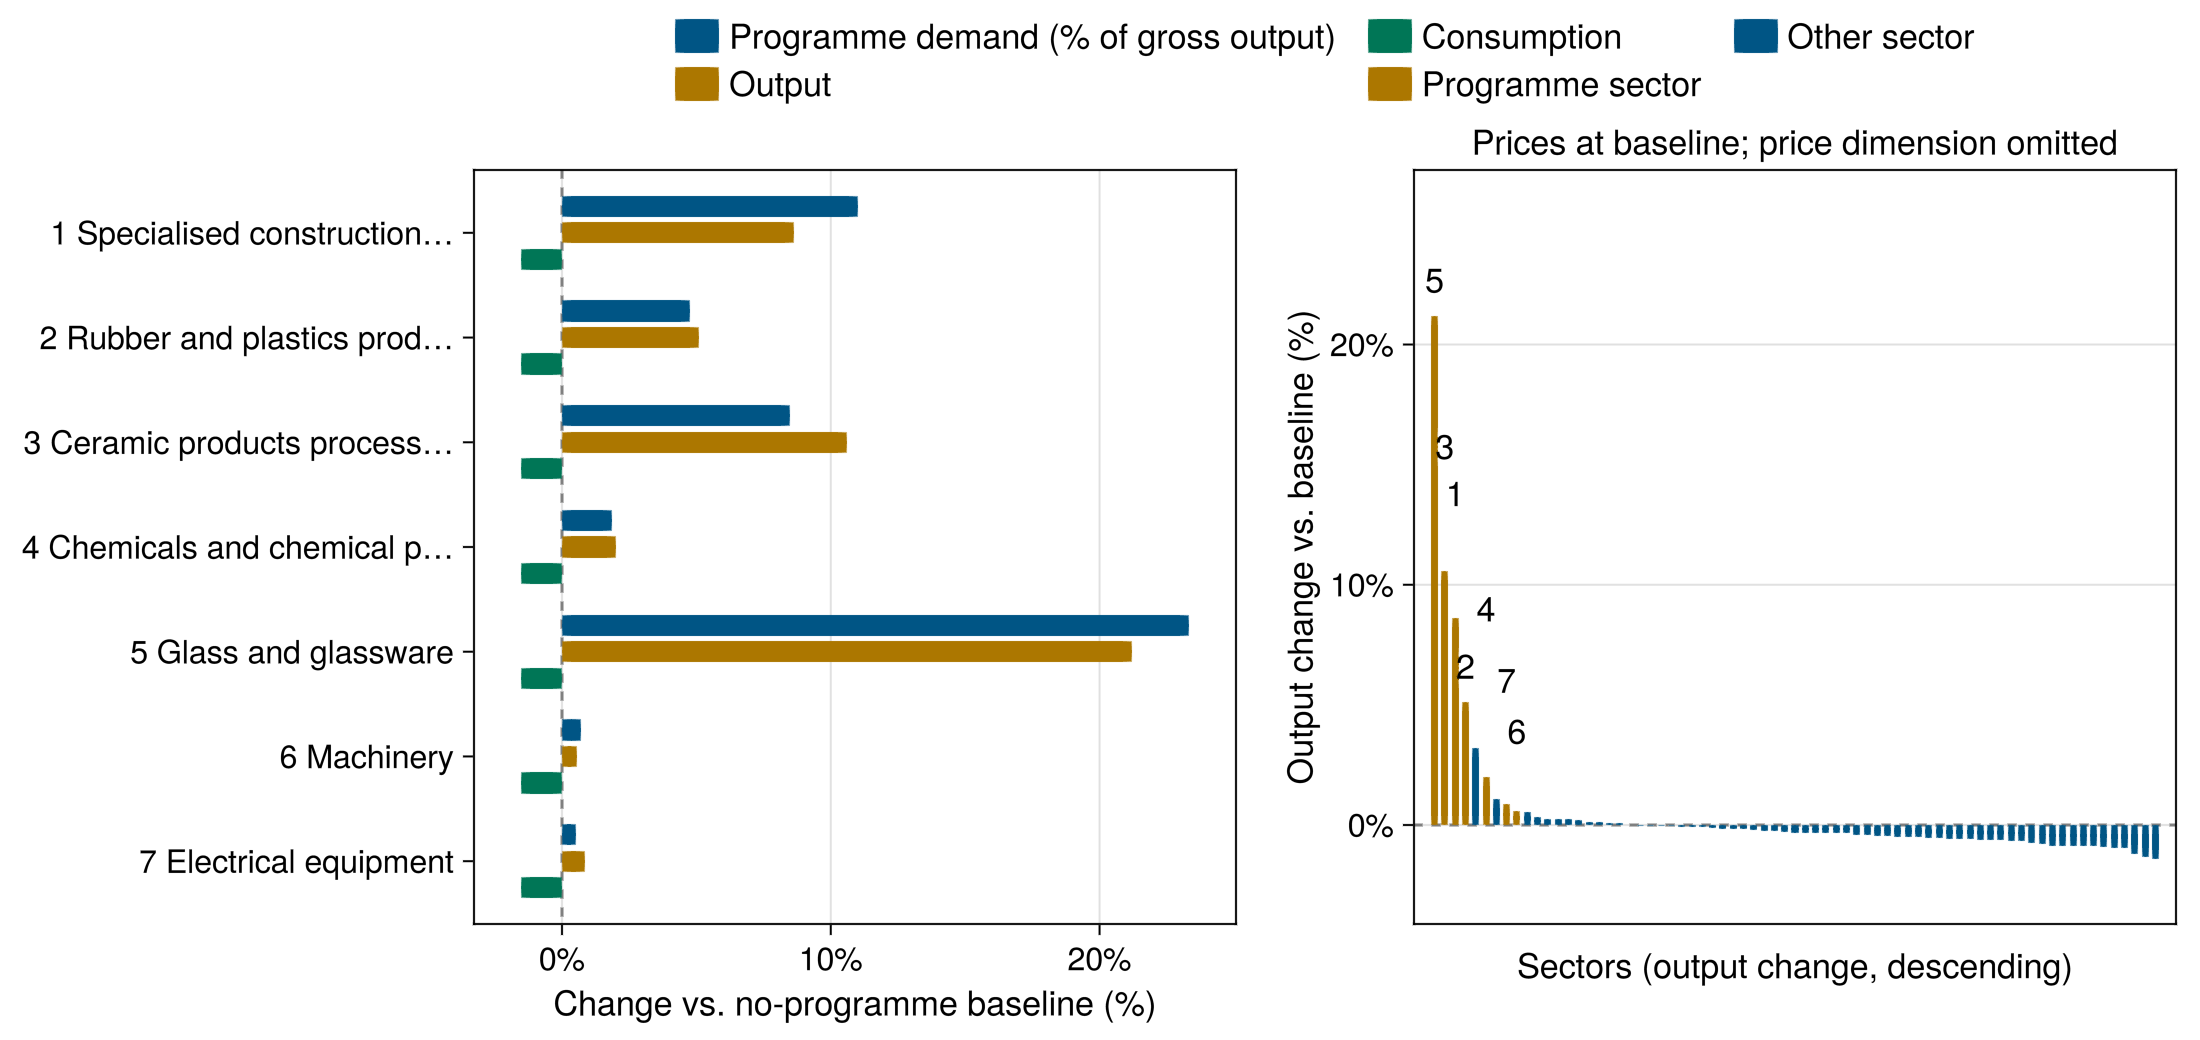
\includegraphics[width=\textwidth]{images/panel_5x3_GAMMA_F2.png}
\caption{Employment adjustment / Leontief, F2}
\end{subfigure}
\begin{subfigure}{0.9\textwidth}
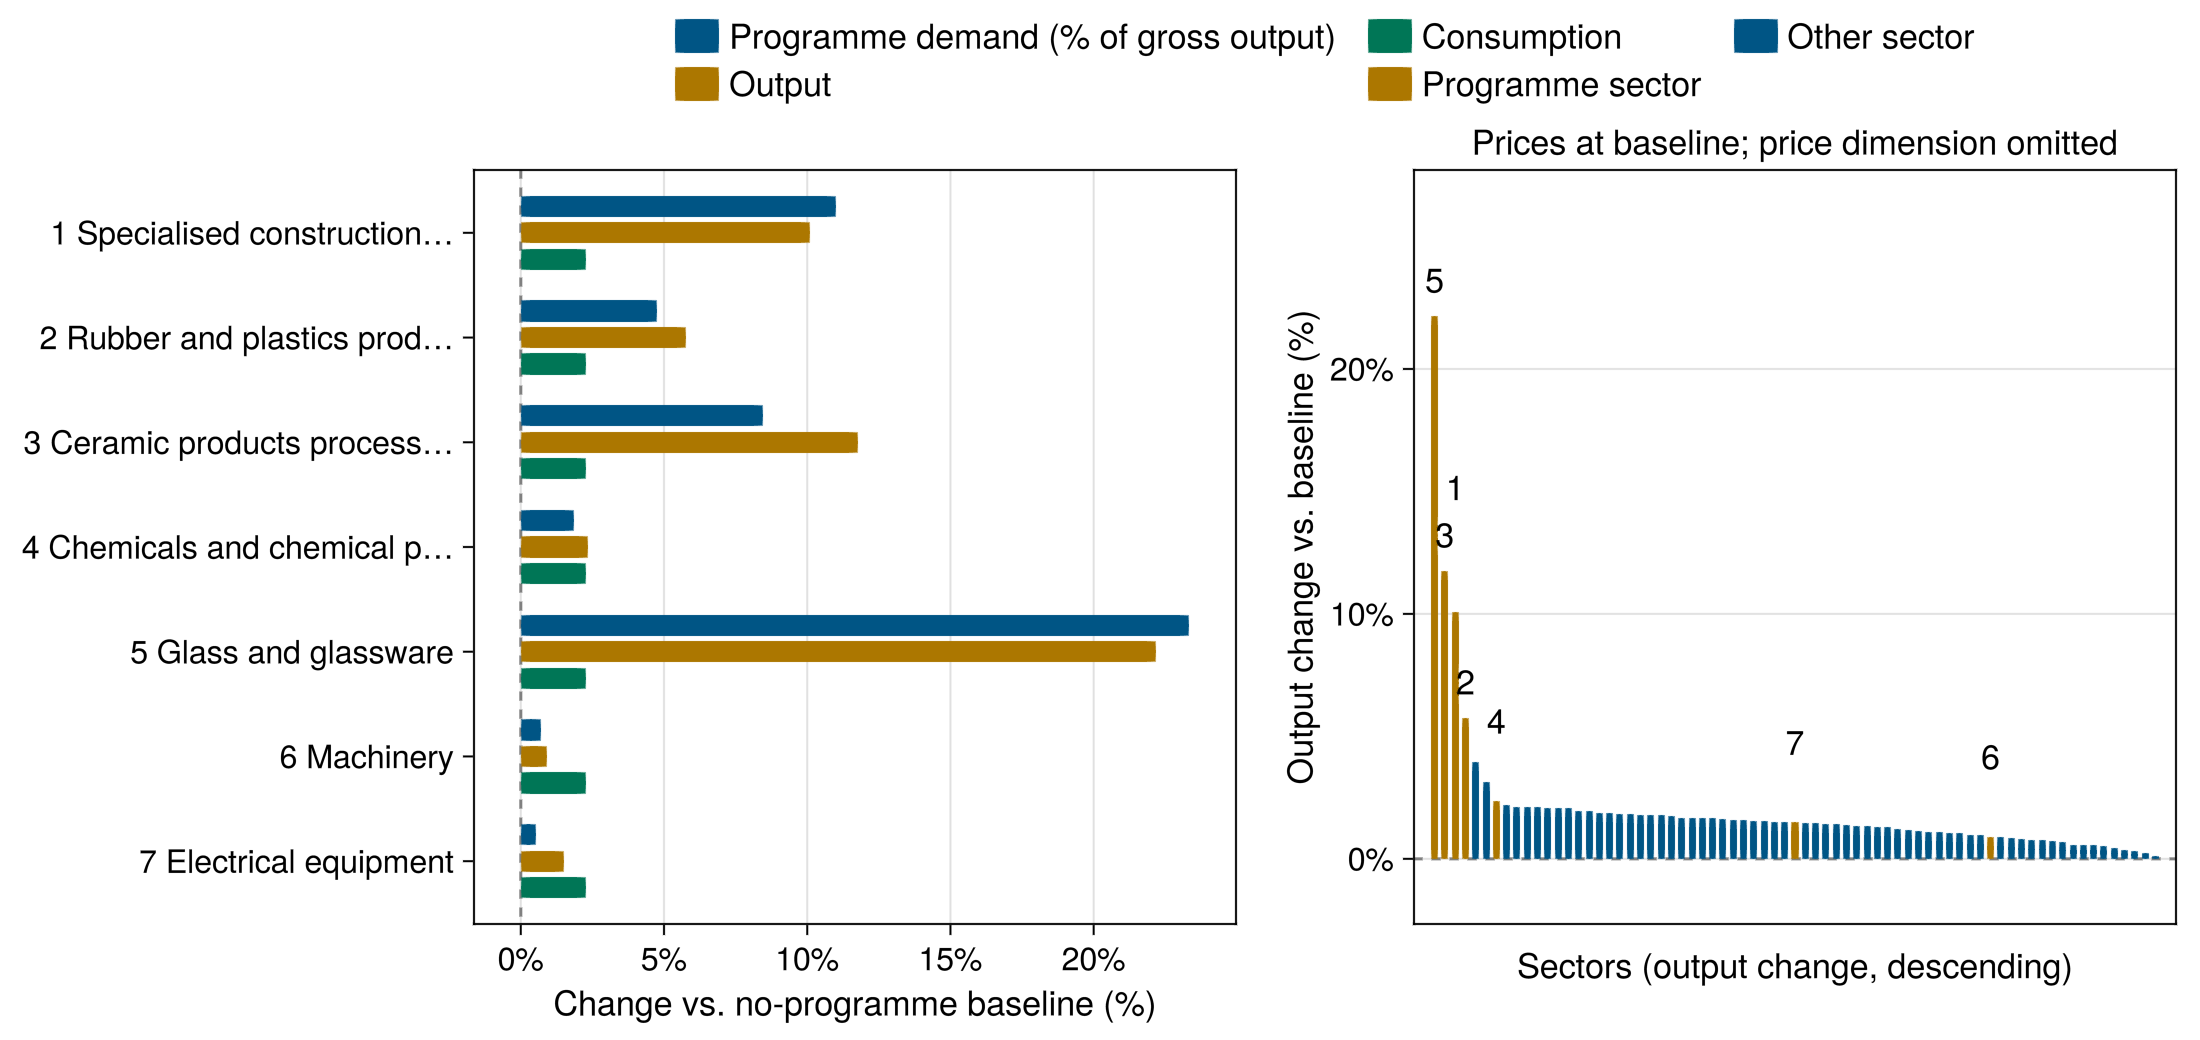
\includegraphics[width=\textwidth]{images/panel_5x3_GAMMA_F3.png}
\caption{Employment adjustment / Leontief, F3}
\end{subfigure}
\caption{Sectoral responses in the coincident employment-adjustment and Leontief closures. Layout as in Figure~\ref{fig:sectoral-flex-f23}; prices remain at baseline, so the right half ranks sectors by output.}
\label{fig:sectoral-fixed}
\end{figure}
